 \documentclass[rgb]{beamer}
\usepackage{silence,lmodern}
\usepackage[backend=biber, style=nature]{biblatex}
\usepackage{csquotes}
\usepackage{listings}
\usepackage{svg}
\usepackage{multirow}
\usepackage{booktabs}
\usepackage{multicol}
\usepackage{forest}
\usepackage[format=plain, justification=justified, labelfont=bf, textfont=it, font=small, labelsep=space]{caption}
\usepackage{appendixnumberbeamer}

\WarningFilter{biblatex}{Patching footnotes failed}
\WarningFilter{etex}{Extended allocation already in use}

\renewcommand*{\bibfont}{\tiny}
\bibliography{ressources.bib}

\usetheme{Konstanz}
\setcounter{secnumdepth}{3}
\format{169}


\title{Label Hierarchy Inference in Property Graph Databases}
\titleCorporateDesign{Label Hierarchy}{Inference in}{Property Graph}{Databases}
\author{Fabian Klopfer} 
\date{10.03.2020}
\institute{Databases and Information Systems Group \\ University of Konstanz}

\AtBeginDocument{
\usebeamerfont{normalfont}
\begin{frame}
	\titlepage
\end{frame}
}

\begin{document}
  \begin{frame}<beamer>
    \frametitle{Outline}
    \tableofcontents[subsectionstyle=hide]
  \end{frame}
  
\section{Introduction}
    \subsection{Motivation}
    \begin{frame}{Motivation}
        \begin{center}
            \textit{``Thus my central theme is that complexity frequently takes the form of hierarchy and that hierarchic systems have some common properties, independent of their specific content. Hierarchy, I shall argue, is one of the central structural schemes, that the architect of complexity uses.``} \\
            \vspace{0.3cm}
            - Herbert A. Simon, \\
            Nobel Laureate and ACM Turing award winner, \\
            The Sciences of the Artificial, 1968~\cite{simon2019sciences}. \\
        \end{center}{}
        \vspace{1.5cm}
        \begin{itemize}
            \item Implicit hierarchical structure in many data sets
            \item Implicit in database models
            \item No explicit representation in the property graph model or Neo4J
        \end{itemize}        
    \end{frame}
    
    \subsection{Problem Statement}
    \begin{frame}[fragile]{Problem Statement}
        \begin{multicols}{2}
            \textbf{Given:} Data set represented in the property graph model \\
            \textbf{Wanted:} Hierarchy of labels reflecting the implicit hierarchical structure \\
            \vspace{0.8cm}
            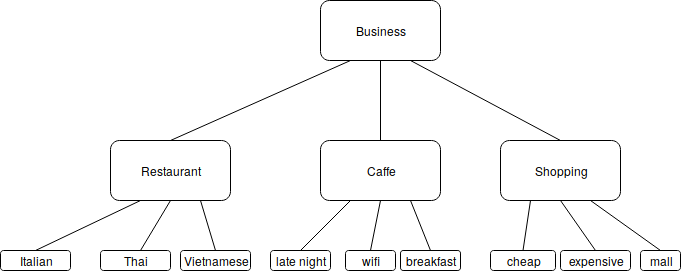
\includegraphics[keepaspectratio,width=\columnwidth]{img/ex_hierarchy.png} \\
            \vfill\null
            \columnbreak
            \begin{tabular}{c c} \toprule
                 Node.name & Node.tags \\ \midrule
                Fernando's & restaurant, italian \\ 
                Arche & restaurant, vietnamese \\ 
                Bangkok & restaurant, thai \\ 
                CampusCafe & cafe, wifi \\ 
                Endlicht & cafe, latenight \\ 
                Pano & cafe, breakfast \\ 
                Lago & shopping, mall \\ 
                Seerhein Center & shopping, cheap \\ 
                Seepark & Shopping, expensive \\ \bottomrule
            \end{tabular}
        \end{multicols}
    \end{frame}

    \subsection{Pipeline}
    \begin{frame}{Overview}
        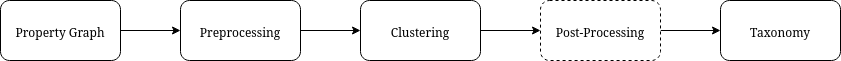
\includegraphics[keepaspectratio,width=\textwidth, height=0.7\textheight]{img/pipeline.png}
        \vspace{2cm}
        \begin{itemize}
            \item Pre-Processing: Feature Generation \& String Vectorization
            \item Post-Processing: Dendrogram flattening
            \item Steps vary between algorithms
            \item For some additional parameter inference necessary: Randomized search used here
        \end{itemize}
    \end{frame}
    
\section{Survey}
    \begin{frame}
        \sectionpage
        \textbf{Goal:} Qualitative and quantitative evaluation of different approaches. \\ \vspace{0.7cm}
        \begin{itemize}
            \item Quality: Deviation from synthetic ground truth
            \item Quantity: Memory and run time complexity, benchmarked run time of state of the art implementations
        \end{itemize}
        \vspace{0.7cm}
        Approaches considered in this thesis: \\ \vspace{0.3cm}
        \begin{enumerate}
            \item Agglomerative Clustering~\cite{Ward1963HierarchicalGT}
            \item Two-Step: Non-Hierarchical and Agglomerative Hierarchical Clustering~\cite{mcinnes2017hdbscan}
            \item Conceptual Clustering~\cite{michalski1980knowledge}
        \end{enumerate}
    \end{frame}
    
    \subsection{Algorithms}
        \begin{frame}{Hierarchical Agglomerative Clustering}
            \begin{multicols}{2}
                \begin{itemize}
                    \item  Basic Idea:
                    \begin{enumerate}
                        \item compute the pairwise distance matrix
                        \item Merge the two clusters with the smallest cluster distance.
                    \end{enumerate}
                    \item Computational Complexity: $\mathcal{O}(n^3)$            
                    \item Space Complexity: $\mathcal{O}(n^2)$
                    \item Extension with a computational complexity of $\mathcal{O}(n^2)$: Robust Single Linkage~\cite{Chaudhuri2010RatesOC}          
                \end{itemize}
                \vfill\null
                \columnbreak
                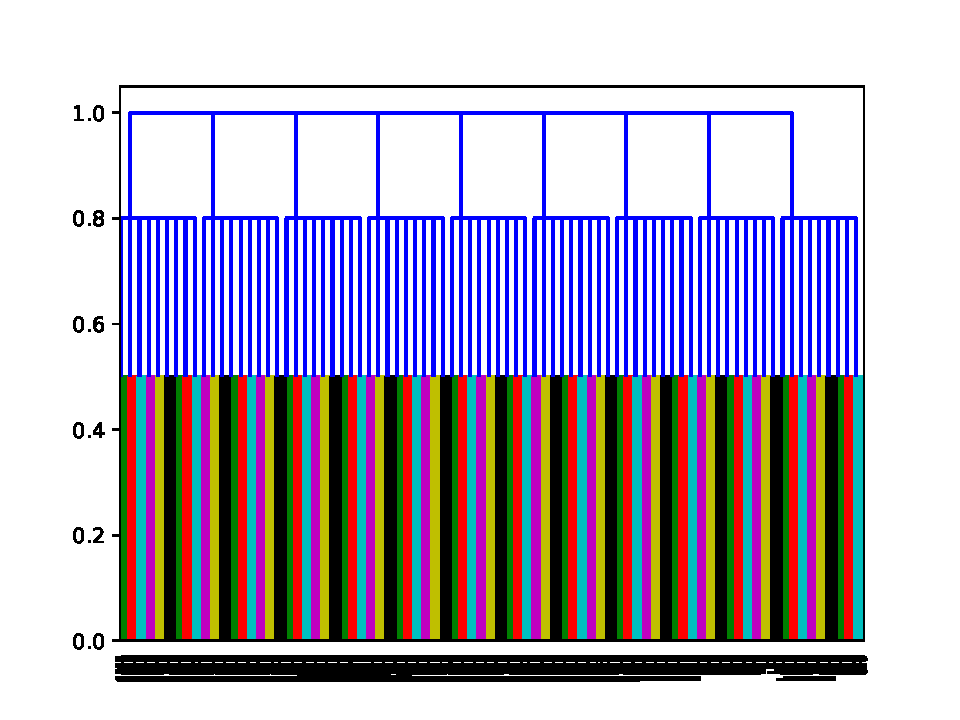
\includegraphics[keepaspectratio,width=\columnwidth, height=0.7\textheight]{img/linkage/synth_noise_0_dendro.pdf}
            \end{multicols}
        \end{frame}
        
        \begin{frame}{Two-step clustering}
            \begin{itemize}
                \item  Basic Idea: Apply a ``flat`` clustering algorithm and combine it with subsequent hierarchical clustering. \\
                \item Partition-based: k-Means, TTSAS~\cite{macqueen1967some, THEODORIDIS2009627}
                \item Density-based: DBSCAN, OPTICS, HDBSCAN~\cite{dbscan, optics, mcinnes2017hdbscan}
                \item requires to infer parameters of the flat clustering algorithms
            \end{itemize}
           
            \centering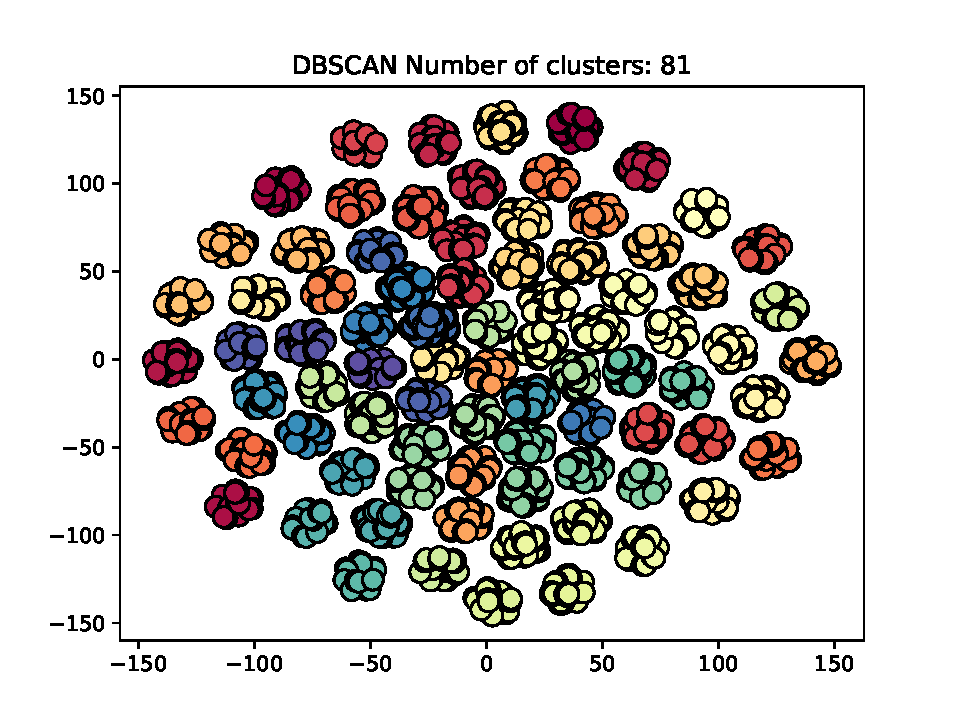
\includegraphics[keepaspectratio,width=\textwidth, height=0.5\textheight]{img/dbscan/synth_noise_0_clusters.pdf}  \hspace{1.5cm}
            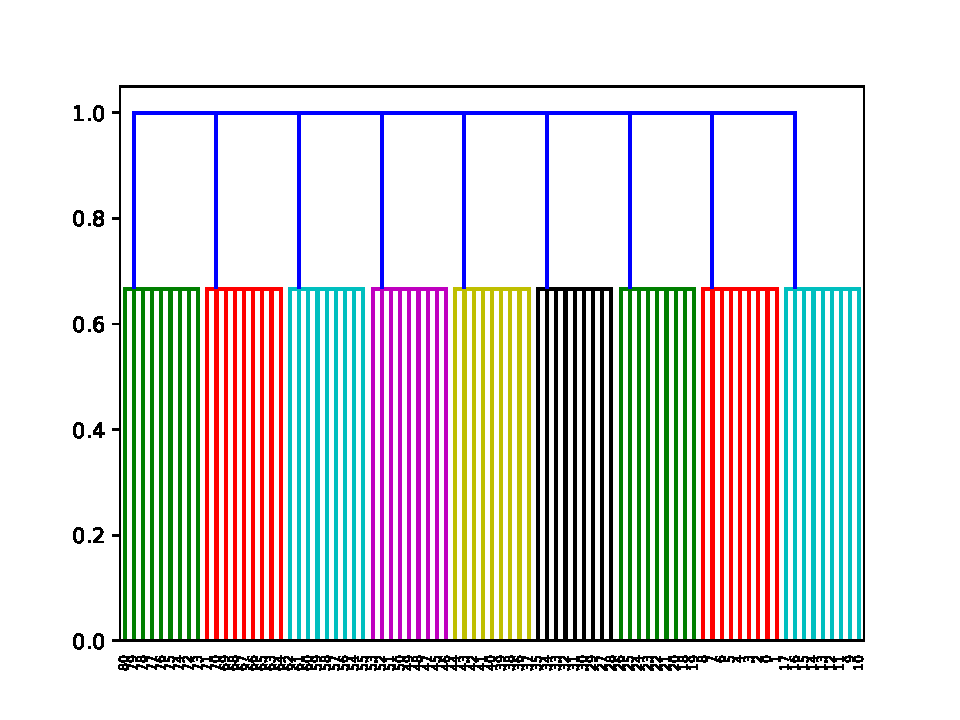
\includegraphics[keepaspectratio,width=\textwidth, height=0.5\textheight]{img/dbscan/synth_noise_0_dendro.pdf}
        \end{frame}
    
        \begin{frame}{Conceptual clustering}
            \begin{itemize}
                \item Basic Idea: Build a hierarchy of label sets/concepts with descriptions by integrating instances iteratively
                \item When integrating choose one of five operations at each level, optimizing value-predictiveness~\cite{gennari1989models, mckusick1990cobweb, corter1992explaining, gluck1985information}
            \end{itemize}
            \centering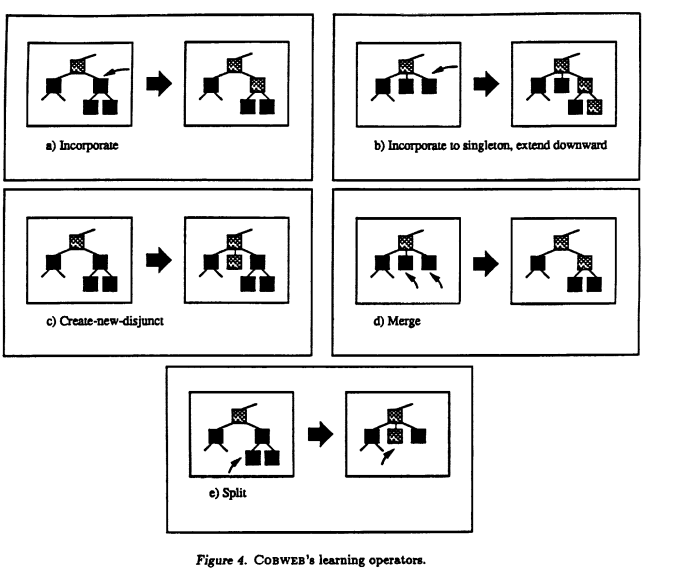
\includegraphics[keepaspectratio,width=0.48\textwidth,height=0.6\textheight]{img/cobweb_ops.png} \hspace{2cm}
            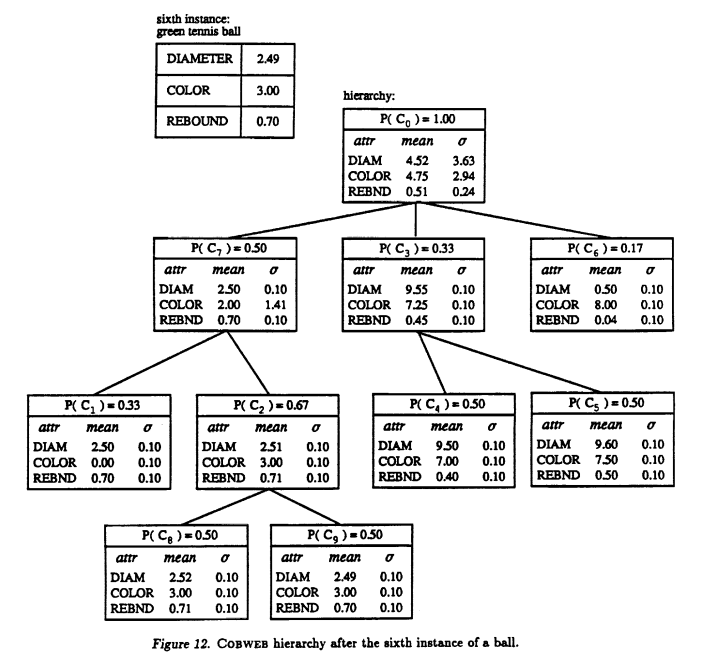
\includegraphics[keepaspectratio,width=0.48\textwidth,height=0.6\textheight]{img/cobweb_ex.png}
        \end{frame}
    
        \begin{frame}{Summary Algorithms}
            \centering
            \begin{tabular}{c c c} \toprule
                Algorithm & Runtime Complexity & Space Complexity  \\ \midrule
                Single Linkage & $\mathcal{O}(n^3)$ & $\mathcal{O}(n^2)$ \\
                Robust Single Linkage & $\mathcal{O}(n^2)$ & $\mathcal{O}(n^2)$ \\
                k-Means & $\mathcal{O}(n \cdot k \cdot d \cdot i)$ & $\mathcal{O}(n)$ \\
                TTSAS & $\mathcal{O}(n^2)$ & $\mathcal{O}(n)$ \\
                DBSCAN & $\mathcal{O}(n \cdot \log(n))$ & $\mathcal{O}(n^2)$ \\
                OPTICS & $\mathcal{O}(n \cdot \log(n))$ & $\mathcal{O}(n^2)$ \\
                HDBSCAN & $\mathcal{O}(n^2)$ & $\mathcal{O}(n^2)$ \\
                COBWEB & $\mathcal{O}(n \cdot \log (n) \cdot b^2 AV)$ & $\mathcal{O}(n)$ \\ \bottomrule
            \end{tabular}
        \end{frame}
    
    \subsection{Experimental Evaluation Setup}
        \begin{frame}[fragile,allowframebreaks]{Experimental Evaluation Setup}
            \begin{itemize}
                \item A synthetic data set is used
                \item noise $\equiv$ take a node and remove $\vee$ rename a label. \\
                \begin{lstlisting}
                "id":24,"labels":"l2, l22",
                "id":25,"labels":"l22",
                "id":26,"labels":"l1"
                \end{lstlisting}
                \item Run the pipeline on each of the noise variations and algorithm:
                \begin{itemize}
                    \item no noise
                    \item $5\%$ noise
                    \item  $10\%$ noise
                    \item $20\%$ noise
                    \item $33\%$ noise
                \end{itemize} 
                \item $\dots$ and for each of the sample sizes
                \begin{table}[htp]
                     \centering
                     \begin{tabular}{ r r r} \toprule
                            Size & Width & Depth \\ \midrule
                            243 & 3 & 5 \\
                            512 & 8 & 3 \\
                            1024 & 4 & 5 \\
                            1331 & 11 & 3 \\
                            1728 & 12 & 3 \\
                            2197 & 13 & 3 \\
                            2401 & 7 & 4 \\
                            3125 & 5 & 5 \\
                            4096 & 4 & 6 \\
                            6561 & 9 & 4 \\ \bottomrule
                        \end{tabular}
                    \caption{The parameters used during evaluation in the synthetic data generator.}
                    \label{tab:synthetic_params}
                \end{table}{}
                \item  Metric for how much resulting hierarchy deviates from perfect: Tree Edit Distance \cite{pawlik2011rted} \cite{pawlik2016tree} 
            \end{itemize}
        
            \begin{itemize}
                \item Implementation of the algorithms: SciPy \cite{scipy}, scikit-learn \cite{scikit-learn}, PyClustering \cite{Novikov2019}, concept-formation \cite{trestle:2016a}, hdbscan \cite{mcinnes2017hdbscan}. 
                \item For all algorithms having parameters: Use Random Search-based parameter optimization (32 Samples)
            \end{itemize}
        \end{frame}
        
    \subsection{Results}
        \begin{frame}[allowframebreaks]{Survey Results}
            \centering 
            \begin{tikzpicture}
                \begin{axis}[
                    title=Quantitative Result,
                    width=0.5\textwidth,
                    height=0.7\textheight,
                    legend pos=outer north east,
                    legend style={draw=none},
                    axis lines = left,
                    ymax = 1000.0,
                    xlabel = Samples,
                    ylabel = Runtime in s,
                    grid=major,
                    legend entries={DBSCAN,HDBSCAN,k-Means, OPTICS, RobustSingleLinkage, SingleLinkage, Trestle, TTSAS},
                    %xtick=data
                ]
                    \addplot [red, mark=x] file {data/part1/rt/synth_DBSCAN_rt.dat};
                    \addplot [blue, mark=square] file {data/part1/rt/synth_HDBSCAN_rt.dat};
                    \addplot [green, mark=*] file {data/part1/rt/synth_KMeansWrapper_rt.dat};
                    \addplot [black, mark=triangle] file {data/part1/rt/synth_OPTICS_rt.dat};
                    \addplot [cyan, mark=diamond] file {data/part1/rt/synth_RobustSingleLinkage_rt.dat};
                    \addplot [teal, mark=o] file {data/part1/rt/synth_SingleLinkage_rt.dat};
                    \addplot [brown, mark=square*] file {data/part1/rt/synth_Trestle_rt.dat};
                    \addplot [magenta, mark=+] file {data/part1/rt/synth_TTSASWrapper_rt.dat};
                \end{axis}
            \end{tikzpicture}
            \centering
            \begin{tikzpicture}
                \begin{axis}[
                    title=Qualitative Results,
                    width=0.5\textwidth,
                    height=0.7\textheight,
                    legend pos=outer north east,
                    legend style={draw=none},
                    axis lines = left,
                    xlabel = Noise,
                    ylabel = $\frac{\text{Tree Edit Distance}}{|\text{samples}|}$,
                    grid=major,
                    legend entries={DBSCAN,HDBSCAN,k-Means, OPTICS, RobustSingleLinkage, SingleLinkage, Trestle, TTSAS},
                    %xtick=data
                ]
                    \addplot [red, mark=x,samples=5] file {data/part1/ted/DBSCAN_ted_norm.dat};
                    \addplot [blue, mark=square, samples=5] file {data/part1/ted/HDBSCAN_ted_norm.dat};
                    \addplot [green, mark=*, samples=5] file {data/part1/ted/KMeansWrapper_ted_norm.dat};
                    \addplot [black, mark=triangle, samples=5] file {data/part1/ted/OPTICS_ted_norm.dat};
                    \addplot [cyan, mark=diamond, samples=5] file {data/part1/ted/RobustSingleLinkage_ted_norm.dat};
                    \addplot [teal, mark=o, samples=5] file {data/part1/ted/SingleLinkage_ted_norm.dat};
                    \addplot [brown, mark=square*, samples=5] file {data/part1/ted/Trestle_ted_norm.dat};
                    \addplot [magenta, mark=+, samples=5] file {data/part1/ted/TTSASWrapper_ted_norm.dat};
                \end{axis}
            \end{tikzpicture}
        \end{frame}{}
    
    \subsection{Discussion}
    \begin{frame}
        \subsectionpage
            \begin{itemize}
                \item Performance of hierarchical agglomerative clustering can be improved by pre-clustering
                \item Parameters vary a lot between data sets and inference is very expensive
                \item TTSAS and k-Means run time highly dependent on parameters and initialization
                \item Density-based methods robust to noise and decent in run time but require additional processing
                \item squared space complexity is infeasible for larger data sets with many features, labels and properties
                \item but can be overcome using database-oriented implementations
                \item empty intersection in noisy domains
                \item Conceptual Clustering can be improved in quality~\cite{fisher1996iterative}, space and computational complexity
            \end{itemize}
        \end{frame}
    
\section{Feature Generation and Selection}
    \begin{frame}{Feature Generation and Selection}
        \textbf{Given:} Data set represented in property graph model  $G = (V, E, \lambda, P, T, L, f_P, f_T, f_L)$ \\
        \textbf{Wanted:} Feature vector capturing graph-based information \\
        \textbf{Possible Features:}
        \begin{itemize}
            \item labels $V, L, f_l$
            \item properties $V, E, P, f_P$,
            \item per node structural features:~\cite{henderson2011s, henderson2012rolx} 
            \begin{itemize}
                \item node degree
                \item average neighbour degree
                \item number of edges incoming to the ego net
                \item number of edges outgoing from the ego net
            \end{itemize}
            \item characteristic set: all connected relationship types $E, T, f_T$ per node~\cite{neumann2011characteristic}
        \end{itemize}
    \end{frame}
    
    \subsection{Experimental Evaluation Setup}
        \begin{frame}{Experimental Evaluation Setup}
        \begin{itemize}
            \item COBWEB is used as algorithm to experiment with as it
            \begin{itemize}
                \item is parameter-free.
                \item requires linear space.
                \item uses probabilistic concepts.
                \item is hierarchical avoiding additional steps.
                \item is able to deal with mixed data.
            \end{itemize}
            \item The LDBC social network benchmark and New York road network data sets are used
            \item Neo4j was used as property graph database, Cobweb was implemented as front-end procedure
        \end{itemize}
        \end{frame}
        
        \begin{frame}{LDBC SNB Schema}
        \centering
        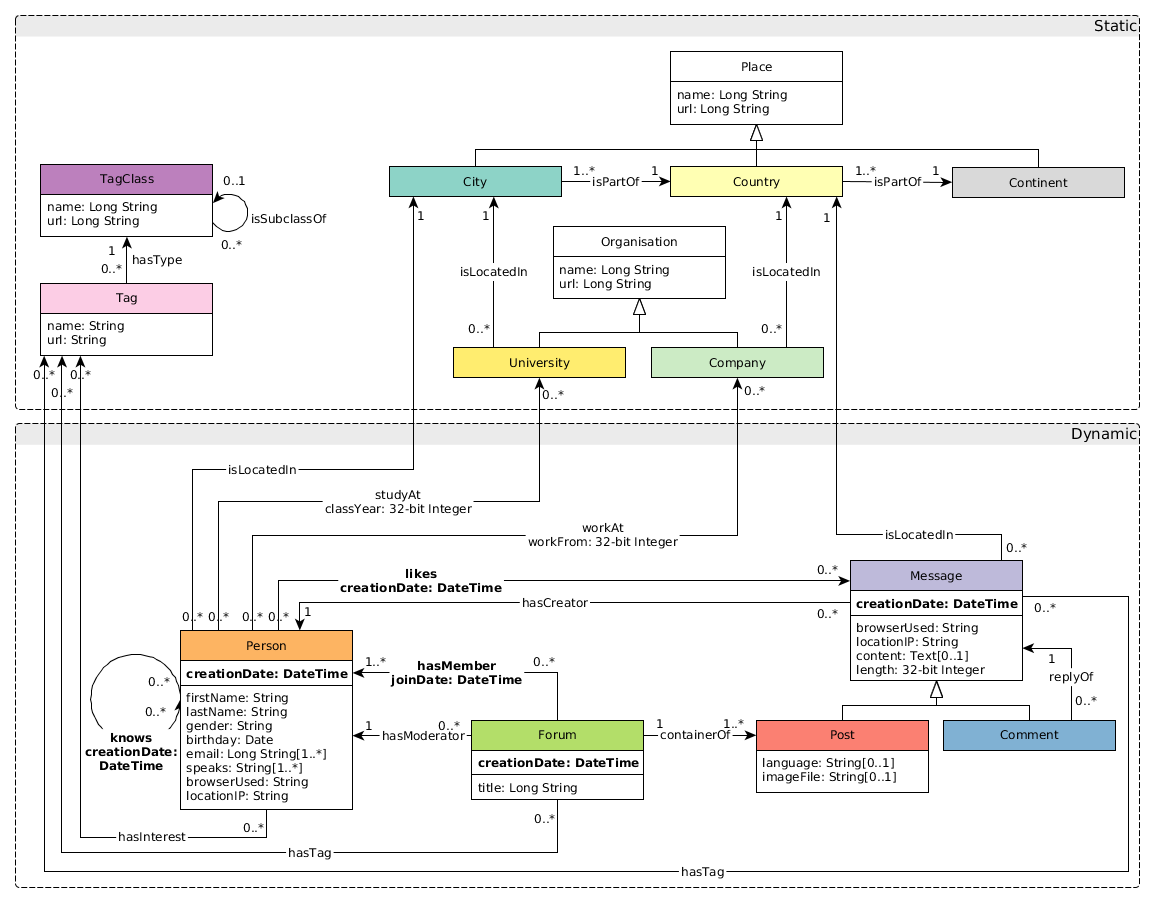
\includegraphics[keepaspectratio,width=\textwidth, height=0.95\textheight]{img/ldbc_snb.png}
        \end{frame}
 
    \subsection{Results}
        \begin{frame}[allowframebreaks]{Results}
            \begin{multicols}{2}
                \begin{itemize}
                    \item Feature Vector of the survey
                    \item Hierarchy splits always nodes with the most frequently occurring label
                \end{itemize}
            \vfill\null
            \columnbreak
                \begin{figure}[htp]
                    \centering
                    \begin{forest}
[Root
	[l0 
		[l00 
]		[l01 
]]	[l1 
		[l10 
]		[l11 
]]]
\end{forest} 
                    \caption{LDBC SNB: labels only}
                \end{figure}{}
            \end{multicols}
            \begin{table}[H] 
                 \begin{longtable}{|c|c|c|c|c|} \hline 
                    Attribute & ValueType & Value & Probability & Occurences \\ \hline 
                    \multirow{2}{*}{Labels} & Nominal & Message & $1.0000$ & $1289$ \\ \cline{2-5} 
                     & Nominal & Comment & $1.0000$ & $1289$ \\ \hline 
                 \caption{Example concept description for node l0: P(node) = 0.6445, Count = 1289}\label{l0ex}
                \end{longtable}
            \end{table} 
         
             \begin{itemize}
                 \item Adding properties, adds further refinements (e.g. splits on length for messages)
                 \item Depending on the format and number of properties
             \end{itemize}
             \begin{figure}[htp]
                \centering
                 \begin{forest}
[Root
	[l0 
		[l00 
]		[l01 
]]	[l1 
		[l10 
]		[l11 
]]]
\end{forest}
                \caption{LDBC SNB: labels and properties}
            \end{figure}{}
        \framebreak
        
             \begin{itemize}
                 \item Using labels, structural features and the characteristic set supports road net-like data sets
                 \item Especially useful if labels, relationship types and properties are uniform, non-existing or noise
                 \item Hierarchy induces distinct connectivity profiles within neighbourhood for road net
             \end{itemize}
             \begin{figure}[htp]
                \centering
                \begin{forest}
[Root
	[l0 
		[l00 
]		[l01 
]]	[l1 
		[l11 
]]	[l2 
		[l20 
]		[l21 
]		[l22 
]		[l23 
]		[l24 
]]]
\end{forest}
                \caption{New York road net: labels, structural features and characteristic set}
            \end{figure}{}
        \framebreak 
        
            \begin{itemize}
                \item Separates by label message at first split
                \item On the second, divides messages into those with low degree and high degree with characteristic sets being IS\_COMMENT\_OF, HAS\_TAG on the high degree side with 
                \item on the other branch of the tree posts are being split from the rest of the nodes
            \end{itemize}
            \begin{figure}[htp]
                \centering
                \begin{forest}
[Root
	[l0 
		[l00 
]		[l01 
]]	[l1 
		[l10 
]		[l11 
]]]
\end{forest}
                \caption{LDBC SNB: labels, structural features and characteristic set}
            \end{figure}{}
        \framebreak
        
            \begin{itemize}
                \item Using all available features introduces noise, depending on the amount of overall information in the features
                \item here the second level split now clusters messages that were created using the same browser
            \end{itemize}
            \begin{figure}[htp]
                \centering
                \begin{forest}
[Root
	[l0 
		[l00 
]		[l01 
]]	[l1 
		[l10 
]		[l11 
]]]
\end{forest}
                \caption{LDBC SNB: labels, properties, structural features and characteristic set}
            \end{figure}{}
        \end{frame}
        
    \subsection{Discussion}
        \begin{frame}{Discussion: Feature Vector}
        Property graph model allows many ways of representing data: \\ \vspace{0.2cm}
            \begin{itemize}
                \item \textit{OO-like} Many node labels, many node properties, no relationships at all \\
                $\Rightarrow$ Labels and properties \\ \vspace{0.3cm}
                \item \textit{RDF-like} Many labels, many relationship types, no properties \\ 
                $\Rightarrow$ Structural features, labels and characteristic set \\ \vspace{0.3cm}
                \item \textit{More complex} Many labels, many rel. types, many properties for both nodes and relationships, varying structural features \\ 
                $\Rightarrow$ All features carry information, which are the predictive ones? \\ \vspace{0.3cm}
            \end{itemize}
            \textit{Too much information introduces noise, not enough information yields trivial hierarchies} \\
            $\Rightarrow$ \alert{Use adaptive feature vector, depending on the information available in the database profile}
    \end{frame}
    
\section{Conclusion}
    \subsection{Summary}
    \begin{frame}{Summary}
       \begin{itemize}
           \item Classical hierarchical agglomerative clustering does not scale well enough to derive meaningful hierarchies directly 
           \item two-phase approaches improve the performance, but require parameters to be optimized
           \item Conceptual clustering provides parameter-free hierarchical clustering, possibly online and with potential optimizations to scale
           \item Feature Vectors need to be constructed adaptively when possible 
           \item too large ones slow computation down and introduce noise
           \item too small ones do not provide enough information for all data representations in the property graph model
       \end{itemize}
    \end{frame}{}

    \subsection{Future Work}
    \begin{frame}[allowframebreaks]{Cardinality Estimation}
        \begin{itemize}
            \item many databases use independence, and uniformity assumption, database profile, histograms, sampling techniques
            \item Example Neo4j: 
            \begin{enumerate}
                \item The number of nodes having a certain label.
                \item The number of relationships by type.
                \item  The number of relationships by type, ending or starting from a node with a specific label.
                \item Selectivity per index.
                \item One additional index at a time.
            \end{enumerate}
            \item Taxonomies capture differences in value distributions dependent on the description of the concept
            \item Storing taxonomies explicitly as index in the database profile provides more information on the selectivity and conditional covariances between attributes
            \item instead of the whole taxonomy, labels can be used along with the concept description
            \item Query optimizer needs to be adapted to query the index appropriately
            \item Further refinements to COBWEB may help to speed up
            \item Algorithm is incremental in nature (update-able)
        \end{itemize}
    \end{frame}

\section{References}
    \begin{frame}[allowframebreaks]{References}
      \begin{tiny}
      \printbibliography
      \end{tiny}
    \end{frame}
    
\appendix
\begin{frame}{Appendix}
    \centering
    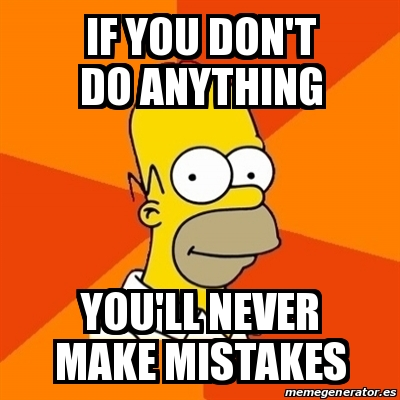
\includegraphics[height=0.85\textheight,width=\textwidth,keepaspectratio]{img/homer.jpg}
\end{frame}
\section{Future Work: Probabilistic Concept Lattices}
    \begin{frame}[allowframebreaks]{Concept Lattices}
        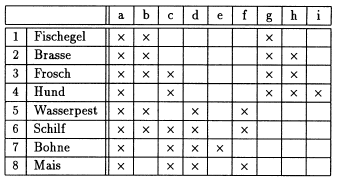
\includegraphics[width=0.48\textwidth]{img/table_hasse.png}
        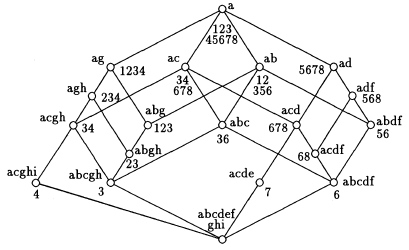
\includegraphics[width=0.48\textwidth]{img/hasse.png}
    \framebreak
        \begin{itemize}
            \item Mathematical framework, developed in the 80s
            \item Able to deal with a wide range of data types (numeric, nominal, ordinal, different scales, $\dots$)
            \item Contains reductions of arbitrary (eventually uncountably infinite) complexity to binary
            \item Has been extended to Fuzzy Concept Lattices for fuzzy sets
            \item Problem: Construction of lattice may end in construction of the power set for independent uniform attribute distributions
        \end{itemize}
    \end{frame}
    
    \begin{frame}{Probabilistic Concepts in a Concept Lattice}
        \textbf{Given:} Attribute A and B are present \\
        \textbf{Desired:} What is the joint distribution for all other non-queried attributes? \\
        \textbf{How does this help us?} 
        \begin{enumerate}
            \item When using all data \\
            \begin{itemize}
                \item Complete analytic characterization pre-computed
                \item One index for all data
                \item maximal linear lookup times for all aggregation queries ($\log_b (2^n)$ assuming $b \geq 2$)
                \item Index-backed property look-up (unclustered)
                \item Exact cardinalities catching all conditional co-variances and conditional selectivities
            \end{itemize}
            \item When sampling from data
            \begin{itemize}
                \item Cardinality estimates incorporating all conditional co-variances
                \item Probably approximately correct learned analytic characterization
            \end{itemize}
        \end{enumerate}
        
    \end{frame}
    
\section{Query Optimization in Neo4j}
    \begin{frame}[allowframebreaks]{Neo4j: Physical Storage}
        \begin{itemize}
            \item Uses offsets as ids
            \item Linked list of fixed size records
            \item Strings and arrays stored separately and dynamically
            \item Nodes and relationships each reference their first property
            \item Nodes reference first relationship of their relationship chain
            \item Relationships reference start and end node, previous and next element in the relationship chain for both start and end node
            \item Indexes consume approximately 1/3 of the average property value size
        \end{itemize}
        \framebreak
        There are three types of files:
        \begin{enumerate}
            \item nodestore.db (node related data; 15B/entry)
            \item relationshipstore.db (relationship related data, 34B/Entry)
            \item propertystore.db (property related data, varies)
        \end{enumerate}
    \end{frame}

    \begin{frame}[allowframebreaks]{Neo4j: Query Processing}
        Steps taken when a query is processed by Neo4j
        \begin{enumerate}
            \item Parse into AST
            \item Optimize and normalize AST into typed AST: \\
            For example move all from MATCH to WHERE
            \item Generate query graph from AST \\
            Also: Retrieve statistics from profile, i.e. label selectivity, index
            \item Create logical plan from query graph
            \item Generate physical/execution plan 
        \end{enumerate}
        \framebreak
        The statistical information that Neo4j keeps is:
        \begin{itemize}
            \item The number of nodes having a certain label.
            \item The number of relationships by type.
            \item The number of relationships by type, ending or starting from a node with a specific label.
            \item  Selectivity per index. (By sampling 5\% after update)
        \end{itemize}
    \end{frame}
    
    \begin{frame}[allowframebreaks]{Example}
        \begin{exampleblock}{Example Cypher Query}
            MATCH (p:Person)-[:LIKES]-(t:Technology) \\
            WHERE p.profession='CS Student' \\
            RETURN p
        \end{exampleblock}
        
        \begin{exampleblock}{Transformed}
            MATCH (p)-[r]-(t) \\
            WHERE p.label='Person', r.type='LIKES', t.label='Technology', p.profession='CS Student' \\
            RETURN p
        \end{exampleblock}
        Now query type hierarchy for node with label Person having relationship of type LIKES and property named profession taking the value 'CS Student'. This can be done in $\log_b (\text{sample size})$.  \\
        \vspace{1cm}
        \begin{itemize}
            \item Should yield a lower cardinality than simply cardinality of label Persons and number relationships by type with start from specific label
            \item Also better than index over Person.profession as relationship type is also taken into account
        \end{itemize}
    \end{frame}
\end{document}